\section{Incremental Filtering and Embedding}
\label{sect:incremental-filtering-and-embedding}

The incremental filtering and embedding phase continues propagating the changes and translates changes of the cluster graph to changes of its filtered graph embedding:
%it takes a sequence of operations that was applied to a cluster graph a
%it takes an old version of a cluster graph $G_\text{old}$ and a sequence of operations $\Delta(G_\text{old}, G_\text{new})$ and output

\begin{figure}[H]
	\centering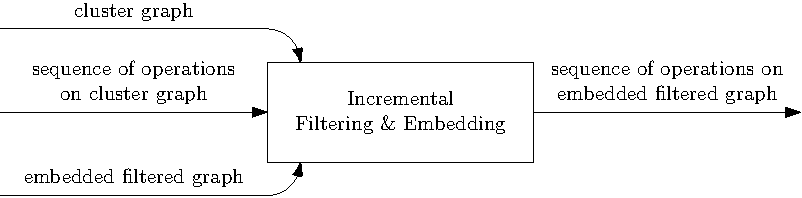
\includegraphics[width=0.9\textwidth]{Resources/DynamicPipeline-IncrementalFilteringAndEmbedding.pdf}
	\caption{Input and output of the incremental filtering and embedding phase.}
	\label{fig:dynamic-pipeline-incremental-filtering-and-embedding}
\end{figure}

Supported operations on embedded filtered graph:
%
\begin{itemize}
	\item change vertex weight
	\item change edge weight
	\item add vertex with arbitrary weight inside an inner face (and connect it to the three vertices of the triangle)
	\item add vertex outside: adjacent to 2 or more vertices on outer face that lie on simple path
	\item remove inner vertex of degree 3
	\item remove outer edge without violating 2-connectedness and internal triangulatedness
	\item add edge on outer face
	\item flip internal edge
\end{itemize}
